% -*-coding: utf-8 -*-
\documentclass[oneside,10pt,a4paper]{article}

\usepackage[utf8]{inputenc}
\usepackage[english]{babel}
\usepackage[IL2]{fontenc}
\usepackage{calc}
\usepackage{graphicx}
\usepackage{booktabs}
\usepackage{multirow}
\usepackage{amsmath}
\usepackage{amsthm}
\usepackage{amstext}
\usepackage{amsfonts}

\setlength{\textwidth}{\paperwidth -5cm}
\setlength{\oddsidemargin}{0cm}
\setlength{\evensidemargin}{0cm}
\setlength{\topmargin}{0cm}
\setlength{\voffset}{-1.7cm}
\setlength{\textheight}{\paperheight -5.6cm}

\newcommand{\beI}{\begin{itemize}}
\newcommand{\enI}{\end{itemize}}
\newcommand{\beE}{\begin{enumerate}}
\newcommand{\enE}{\end{enumerate}}
\newcommand{\Cpp}{C\raisebox{0.15ex}[0ex][0ex]{++}}

\begin{document}
\title{CERN Project Report \\ Development and Testing of VDT - Fast Math Library}

\author{Ladislav Horký \\ Supervisor: Dr. Danilo Piparo}

\date{7 September, 2012}

\maketitle

\section{Preface}
I worked on development and testing of fast math library called VDT. The library contains a set of basic mathematical functions written in such way that they are not IEEE compliant in terms of accuracy but they are faster than their standard library counterparts. Moreover, structure of the code allows the latest compilers as GCC 4.7 to vectorize (therefore parallelize) program execution resulting in additional significant speedup. The VDT is developed as an open source alternative for Intel's commercial Short Vector Math Library (SVML) which is currently used at CERN.

\section{Tasks}
Here follows the list of tasks I had. As the project was easily extended, I list those which I managed to cover at least partially:
\beE
    \item Get familiar with the current project structure
        \beE
            \item auto-vectorization concept
            \item cmake build configuration tool
            \item test modules
            \item \Cpp 11 features used
        \enE
    \item Finish testing tools
        \beE
            \item saving results to file
            \item enhance random number generation
        \enE
    \item Create tool for automated testing of all functions at once
        \beE
            \item both for testing arithmetic and speed performance
            \item make the code easily extensible, maintainable
        \enE
    \item Create a Python script using PyRoot to plot the results
    \item Test VDT against linux libm and Intel SVML in terms of accuracy and time performance
    \item Test another vectorizing library VC [1] and compare the results
        \beE
            \item create a wrapper for VC functions
            \item connect it to our testing suite
        \enE
    \item Try to compile VDT with other compilers (icc, clang) to see, how they vectorize
    \item Port code to GPU and compare performance
        \beE
            \item use NVIDIA CUDA
            \item compare to native CUDA functions
        \enE
\enE

\section{Task processing and comments}
I will now describe project state at the end of summer, pointing out parts I contributed to. The whole package is meant to provide the core VDT library and diagnostic tools to test it against arbitrary library in terms of speed and accuracy.

\subsection{Structure}
The whole project now consists of several distinct parts as shown in the figure:

\begin{figure}[h]\label{structure}
  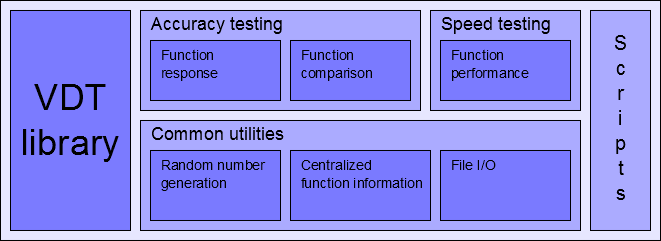
\includegraphics[width = \textwidth]{structure.pdf}
  \caption{Project structure}
\end{figure}

\subsubsection{The library}
The library is completely stand-alone, separately compilable and does not use any \Cpp 11 features for wider compatibility with older compilers. It contains single and double precision functions in two different signatures: single signature with prototype {\tt Type function(Type)} and vector signature {\tt void function(uint,Type*,} {\tt Type*)}. The latter is generated by python script from the single signature and is supposed to auto-vectorize during the compilation. In order to auto-vectorize, function's code must be as linear as possible. That means removing any unnecessary branching, in our case domain checks and special cases check. In addition, Padé approximation is used instead of Taylor using two independent smaller polynomials that can be more aggressively optimized. This part was basically finished when I arrived and only helped with some debugging.

\subsubsection{Utilities}
The rest are parts of the testing suite. Random number generator is based on \Cpp 11 Mersene twister and generates uniform distribution in specified range. I enabled it to generate also piecewise uniform distribution - in our case uniform on $\langle\pm 10^{k-1},\pm 10^k\rangle$ for all $k$ in specified range. In the beginning we considered this useful but it has not been used in testing yet.

To preserve absolute accuracy when saving and loading numbers to and from files, we treat the floating point numbers as hex strings, so the data are saved in exactly the same format as they are held in memory. This is done by two utility classes {\tt fpToHex(Type)} and {\tt fpFromHex()} I created, providing parameterized insertor and extractor for file streams.

There is also a function {\tt getFunctionTuples()} I created, where all the necessary information for all functions tested is held. This makes the set of tested functions easily extensible, as we demonstrated when testing a VC library (see later). The information stored about each function is function name, pointer to the actual function and a random pool of input values from appropriate domain which is enough to perform arbitrary testing.

%I also created a function {\tt getFunctionTuples()} returning a vector of structures containing basic information for each function (name, pointer to the function, input values). Triplets are elegantly implemented using \Cpp 11 {\tt tuple<...>} and are used to easily loop over all functions during testing. Thanks to this, the set of tested functions can be easily extended over other libraries of interest because this is the only place where actual functions and their names come to play. We used this feature to test functions from VC library (see later).

\subsubsection{High level testing suite}
To make scripting more feasible, I wrote or edited all programs in this section so that they have all necessary parameters passed via command line options. Moreover, the (even intermediate) results of programs are stored in files of fixed format for future reference, reuse or backup, as some testing can be very time consuming. It also makes possible to change one piece of testing chain amid testing without need to generate all the intermediate data again. The filenames are automatically generated but contain nickname specified by user via -n option, used for convenience and to distinguish between different test runs.

Files generated by three programs performing tests contain five lines of header holding information about file itself, function name - if appropriate, used precision (single or double) and sometimes some other information. The rest of the file contains, line by line, results for different input values.

\begin{figure}[h]
        \begin{minipage}[l]{0.5\textwidth}
           \center
           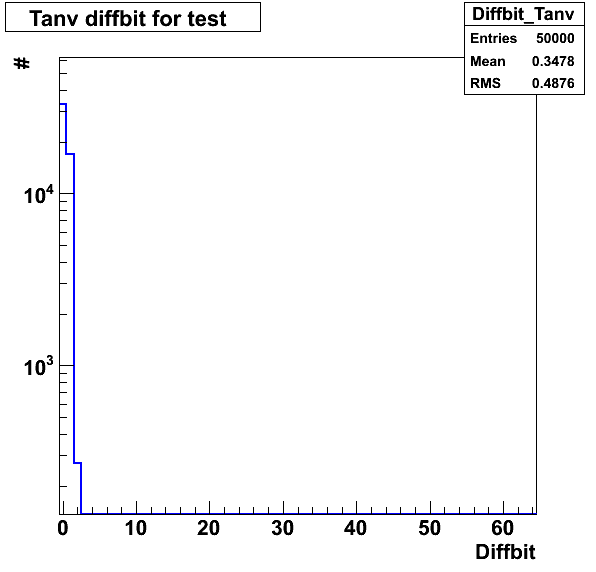
\includegraphics[width=70mm]{diffbit.png}
           \caption{Different bit distribution}
        \end{minipage}
        \begin{minipage}[r]{0.5\textwidth}
            \center
            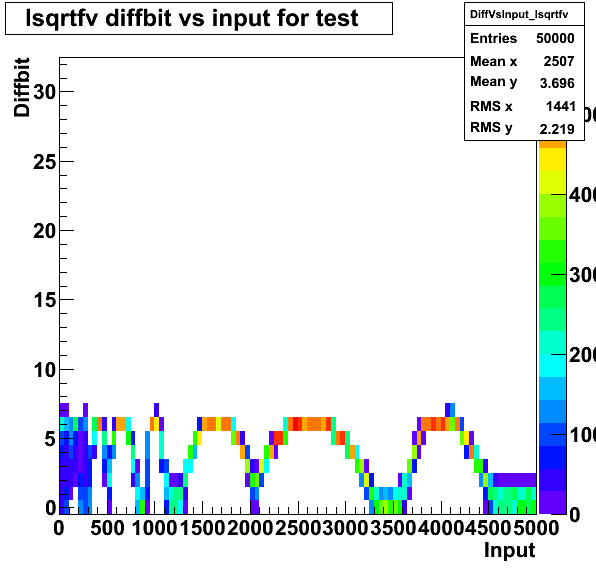
\includegraphics[width=70mm]{inputVSdiffbit.png}
            \caption{Different bit VS input}
        \end{minipage}
        \label{plots}
\end{figure}
The accuracy testing suite consists of two programs. The first, {\tt vdtArithmBenchmark}, saves input and output values of all functions, retrieved by {\tt getFunctionTuples()}, to files. User passes via command line options only a nickname and optionally an amount of test input values. Then user runs {\tt vdtArithmComparison} specifying reference files with -R=$<$comma-separated-list$>$, test files with -T=$<$comma-separated-list$>$ and nickname of output files. The program then pairs the ref and test files in natural manner (1-1, 2-2,...), compares the output values (assuming that corresponding input values are the same) and creates files containing input value, both output values and \emph{most significant different bit} between outputs which is the unit used by us to measure accuracy. Program also prints basic statistics for each function to stdout: max, min different bit, mean and RMS. The files are then processed by a python script, which creates two histograms from each file (Figure 2,3).

The left one serves as a quick reference of how accurate the function is with respect to the others, the right shows distribution of error over the input value range. The latter proved essential for debugging because it showed us few well hidden errors in our functions. Also, for some libraries we tested, these plots were actually first of a kind!

The speed testing is carried out by {\tt vdtPerfBenchmark} and is more straightforward. The tricky part - time measurement itself - was done by my supervisor so I just sewed all pieces together. Program runs all functions for many times with different input values and measures elapsed time. Then prints statistics (mean time, RMS) for each function and saves all results in \emph{one} file.

\subsubsection{Build}
Build of the project is driven by Cmake utility. I wrote the configuration file, so that different build combinations can be chosen via setting cmake cache variables ("{\tt cmake -D VARIABLE=VALUE .}"). Now, following options are possible:
\beI
 \item build library only ({\tt cmake .})
 \item build library together with the testing suite ({\tt cmake -D DIAG=1 .})
 \item choose to use SVML lib instead of standard libm - only at CERN ({\tt cmake -D SVML=1 .})
 \item include VC library in tests ({\tt cmake -D USE\_VC=1 .})
 \item build for a machine which supports AVX instructions ({\tt cmake -D AVX=1 .})
\enI

\subsection{Testing}
Our test were focused on comparing performance of libm and VDT. We also tested the VDT against Intel SVML which uses intrinsics to vectorize and also trades speed for precision. The last test was against
\begin{table}[h]
    \begin{center}
    \begin{tabular}{llllllllll}
      \toprule
      & & \multicolumn{5}{c}{$\!\!\!\!|$\hfill speedup against libm \hfill $|\!\!\!\!$} & \multicolumn{3}{c}{avg. different bit}\\
      Fcn & Libm (ns) & VDT & VDT SSE & VDT AVX & SVML AVX & VC AVX & VDT & SVML & VC\\
      \midrule
    Exp   &16,7& 2,7 & 4,4 & \textbf{5,8} &5,4&X& \textbf{0,14} & 0,43 & X\\
    Log   &34,9& 2,8 & 6,1 & \textbf{8,3} &7,4&6,4& 0,42 & \textbf{0,00} & 0,01\\
    Sin   &33,7& 2,1 & 5,6 & 5,9 &7,8&\textbf{9,4}& \textbf{0,25} & 0,35 & 23,3\\
    Cos   &34,4& 2,6 & 6,4 & 6,7 &7,2&\textbf{11,2}&\textbf{0,25}& 0,35 & 23,3\\
    Tan   &46,6& 3,7 & 7,4 & 8,3 &\textbf{10,0}&X&\textbf{0,35}& 0,49 & X\\
    Asin  &23& 2,2 & 2,7 & 2,8 &3,6&\textbf{4,2}& 0,32 & \textbf{0,24} & 24,3\\
    Acos  &23,7& 2,2 & 2,9 & 2,9 &\textbf{4,0}&X& \textbf{0,39} & 0,79 & X\\
    Atan  &19,7& 1,8 & 2,4 & 2,4 &2,4&\textbf{3,2}& 0,33 & \textbf{0,28} & 2,97\\
    Isqrt &9,3& 1,4 & 3,1 & \textbf{4,4} &X&X& \textbf{0,45} & X    & X\\
      \bottomrule
    \end{tabular}
    \caption{Double precision, results taken from [2]}
    \label{double precision}
    \end{center}
\end{table}
VC library [1] - the function signatures are different than ours, so I created a wrapper to connect it our suite. When USE\_VC is set in cmake, it will propagate to the code as a conditional compilation trigger
and adds VC functions to the set of tested function.
\begin{table}[h]
    \begin{center}
    \begin{tabular}{llllllllll}
      \toprule
      & & \multicolumn{5}{c}{$\!\!\!\!|$\hfill speedup against libm \hfill $|\!\!\!\!$} & \multicolumn{3}{c}{avg. different bit}\\
      Fcn & Libm (ns) & VDT & VDT SSE & VDT AVX & SVML AVX & VC AVX & VDT & SVML & VC\\
      \midrule
Expf&19&2,8&7,6&9,2&\textbf{13,8}&X&3,36&\textbf{0,45}&X\\
Logf&12,6&1,0&5,1&6,6&\textbf{7,8}&5,5&0,26&0,03&\textbf{0}\\
Sinf&180&14,8&66,9&90,0&\textbf{125,0}&\textbf{125,0}&\textbf{0,24}&0,33&9,51\\
Cosf&180&17,8&73,5&105,3&98,9&\textbf{165,1}&\textbf{0,24}&0,33&9,51\\
Tanf&183&14,8&55,3&70,9&\textbf{98,4}&X&\textbf{0,52}&\textbf{0,52}&X\\
Asinf&12,1&1,4&6,1&\textbf{17,0}&5,5&5,9&0,6&0,58&\textbf{0,31}\\
Acosf&14,6&1,5&6,8&\textbf{20,3}&5,7&X&0,48&\textbf{0,4}&X\\
Atanf&10,8&1,8&5,6&\textbf{15,4}&6,0&5,2&\textbf{0,37}&\textbf{0,37}&\textbf{0,37}\\
Isqrtf&9&3,0&15,5&\textbf{21,4}&X&X&\textbf{3,7}&X&X\\
    \bottomrule
   \end{tabular}
    \caption{Single precision, results taken from [2]}
    \label{single precision}
    \end{center}
\end{table}

The speed and accuracy measurement results are summarized in tables \ref{double precision} and \ref{single precision}. The testing setup was following:
\beI
    \item Machine: Intel$^\circledR$Core$^\text{\textsc{TM}}$i7-3930K CPU @ 3.20GHz (AVX support)
    \item Compiler: GCC 4.7, -Ofast turned on for vector signatures compilation
    \item 1 Million numbers repeated 150 times in order to remove statistical fluctuation
    \item Call overhead subtracted using identity function $f(x)=x$
\enI

\subsubsection{Results}
The VC was missing some function and isqrt, as a stand-alone function, was implemented only in VDT. Measurements show that VDT performs well - its speed is comparable to the SVML and accuracy is sufficient for wide range of applications. We can see that VDT functions vectorize quite well as they are closing to the maximal theoretical speedup - in double precision 2x for SSE and 4x for AVX and for single precision 4x for SSE and 8x for AVX (float is half the size of double, so registers can accommodate twice more values).

VC trades speed for precision by using power series from single precision functions even in double precision complements. However, there seems to be an error in range reduction for sin and cos resulting in error growing with input.

\subsubsection{Other compilers}
We planned to do the same tests with different compilers, particularly Intel's icc and open source LLVM-based Clang. Unfortunately I spent most of the time solving incompatibilities arising from their usage with our \Cpp 11 code and we did not manage to do any testing. Few for all: icc is incompatible with GCC 4.7 whose libraries it apparently uses, clang does not understand some \Cpp 11 constructs in GCC libraries and its LLVM optimizer taking care about vectorization is basically undocumented (at least command line options).

\subsubsection{Porting to GPU}
In the end I managed to do some basic tests with porting VDT code to GPU. I wrote a stand alone program which run VDT Exp function on GPU using NVIDIA CUDA and measured its performance against native GPU Exp. Only double precision was tested (in single there was some unknown bug). Code was written in fast copy-paste manner, so no GPU optimizations took place. The tested GPU was NVIDIA GT560 .... Results are summarised in the table below.
\begin{table}[h]
    \begin{center}
    \begin{tabular}{lllll}
      \toprule
    &\multicolumn{2}{c}{speed (ns)}&\multicolumn{2}{c}{accuracy (diff. Bits)}\\
    Function & transfer time & kernel time & average & RMS\\
    \midrule
    VDT Exp&5,25&0,7&0,14&0,12\\
    Cuda Exp&5,25&0,43&0,09&0,09\\
    \bottomrule
    \end{tabular}
    \caption{Quick CUDA test}
    \label{cuda}
    \end{center}
\end{table}

From the results we can see that CUDA Exp is still better than our implementation which, however, performs quite well for copy-pasted code. The next thing is, that most time is taken by transfer of the data than function itself - this brings the thought of computing whole formulas on GPU to minimize transfer overhead. As the the asynchronous communication over PCI Express is involved, measured times vary even for large sets of numbers and many repetitions.

\section{Conclusion}
During the summer we brought the project to the release phase (probably under the LGPL licence) and showed, that the VDT can be the golden choice in terms of speed-precision trade off and extendability (Intel is not open source, VC misses lots of functions). While working on the project, I acquired and improved many useful skills ranging from debugging routines, cmake configuration and python scripting to communication with my supervisor, result presentation and a peek into project management.

\section{References}

[1] VC full description at: {\tt http://code.compeng.uni-frankfurt.de/projects/vc/}\newline
[2] Danilo Piparo: The VDT Mathematical Library presentation \newline
({\tt https://indico.cern.ch/sessionDisplay.py?sessionId=9\&confId=202688\#20120925})\newline
[3] Project's Trac: {\tt https://svnweb.cern.ch/trac/vdt/wiki/WikiStart}


\end{document} 